\documentclass[oneside,a4paper,english,links]{amca}
%
\usepackage{graphicx}
\usepackage{amsmath,amsfonts}
\usepackage[utf8]{inputenc}
%

\usepackage{subcaption} % for creating subfigures
\graphicspath{{Figures/}} % Specifies the directory where pictures are stored
\title{Automating a FEM solution database generation and neural network learning for solid mechanics problems}


\author[a]{L.C. Agorio}
\author[b]{M.C. Vanzulli}
\author[c]{B. Bazzano}
\author[c]{Jorge M. Pérez Zerpa}
%
\affil[a]{Instituto de Ingeniería Eléctrica, Facultad de Ingeniería, Universidad de la República, Montevideo, Uruguay}

\affil[b]{Instituto de Ingeniería Mecánica y Producción Industrial, Facultad de Ingeniería, Universidad de la República, Montevideo, Uruguay}
%
\affil[c]{Instituto de Estructuras y Transporte, Facultad de Ingeniería, Universidad de la República, Montevideo, Uruguay}

\begin{document}
\vspace{3cm}

\maketitle

\begin{keywords}
Artificial Neural Networks, Finite Element Method, Solid Mechanics, Surrogate-models.
\end{keywords}

\begin{abstract}
Solving finite element problems can be computationally expensive, particularly in nonlinear solid mechanics. This challenge emerges in applications such as biomechanics or manufacturing process design, where the same problem may need to be solved in real time for different configurations or input data. In this paper we combine Finite Element Method (FEM) and Artificial Neural Networks (ANN) to improve the speed and efficiency of solvers in solid mechanics problems. A pipeline to generate databases of FEM solutions was developed interacting with an in-house Open Source Software for non-linear Analysis of Structures (ONSAS). The databases were used to train a neural network that takes geometrical and material properties as inputs, and as an output predicts the displacements solution of the mechanical problem. Our experiments showed that the proposed approach was effective, achieving low losses on both the training and test datasets. We present a validation example where the ANN was capable of matching the analytic solution with great accuracy. Moreover, more complex problems were solved with different geometries, boundary conditions and materials, considering large strain deformations. One advantage of our implementation is its simplicity and scalability. We were able to develop a pipeline that can be easily scaled to a wide range of mechanical problems. Additionally, the use of ANN provides a faster computation time than the traditional solvers using the FEM method.  Although the study presents promising results, we also discussed the limitations of the proposed approach and potential directions for future work. 
\end{abstract}

\section{Introduction}
The objective of this project is to develop a surrogate model for unidimensional mechanical problems that is faster than the finite element method (FEM) \citep{martinez2017finite, bohringer2023strategy}. To achieve this, we trained a neural network(NN) using a dataset of FEM solutions to compression/extension mechanical problems. 
%
There is an increasing interest in using this type of models for biological tissues \citep{pellicer2020real}. In this project, we used a FEM solver repeatedly to generate a large dataset of results, which was used to train the NN. 
%
The NN was designed to learn from the FEM solutions and predict the displacement field at particular nodes \cite{yang2022tracker}. Surrogate models can be used for structural assessment by tracking geometric features along time \cite{zhu2023visual} and for solving material identification problems \cite{steuben2015inverse}.
%
Moreover existing methods such as Physics-Informed Neural Networks leverages on the underlying dynamics to train the model \citep{raissi2017physics}. 

This documentation report will describe the methodology used to develop the NN, the performance of the model compared to the FEM, and potential future directions for this project. By developing a faster surrogate model, this project's approach has the potential to significantly improve the efficiency of solving mechanical problems, with broader implications for the engineering design process.

\section{Methodology}
In this section, we describe the pipeline we developed to generate the dataset of FEM solutions and train the NN. We used a simple solid mechanical models with the \texttt{ONSAS.m} FEM solver, which we automated with a bash script. The resulting dataset was preprocessed and used to train a multi-layer perceptron (MLP) implemented in PyTorch.

\subsection{Uniaxial Model}
This model consisted of a uniaxial mechanical problem in which a load was applied to a three-dimensional prism, causing it to deform in three dimensional. The model is uniaxial in the sense that the applied load is along the x-axis. We used the \texttt{ONSAS.m} FEM solver to simulate the deformation and generate a dataset of solutions. The uniaxial model was chosen for its simplicity and as a starting point for more complex models.

The simulated uniaxial problem can be seen in Figure \ref{fig:uniaxial_model}. Loads are applied to the prism at the right end, causing it to deform. The prism is constrained to to mantain the lefmost face (Figure \ref{fig:uniaxial_model}) in the y-z plane, and the origin fixed, thus the deformation is uniaxial.

\begin{figure}[ht]
	\centering
	\begin{subfigure}[b]{0.48\textwidth}
	\def\svgwidth{\textwidth}
	\input{Figures/Example1.pdf_tex}
	\caption{Reference configuration sketch.}
	%\label{fig:image1}
	\end{subfigure}
	\hfill
	\begin{subfigure}[b]{0.48\textwidth}
	\centering
		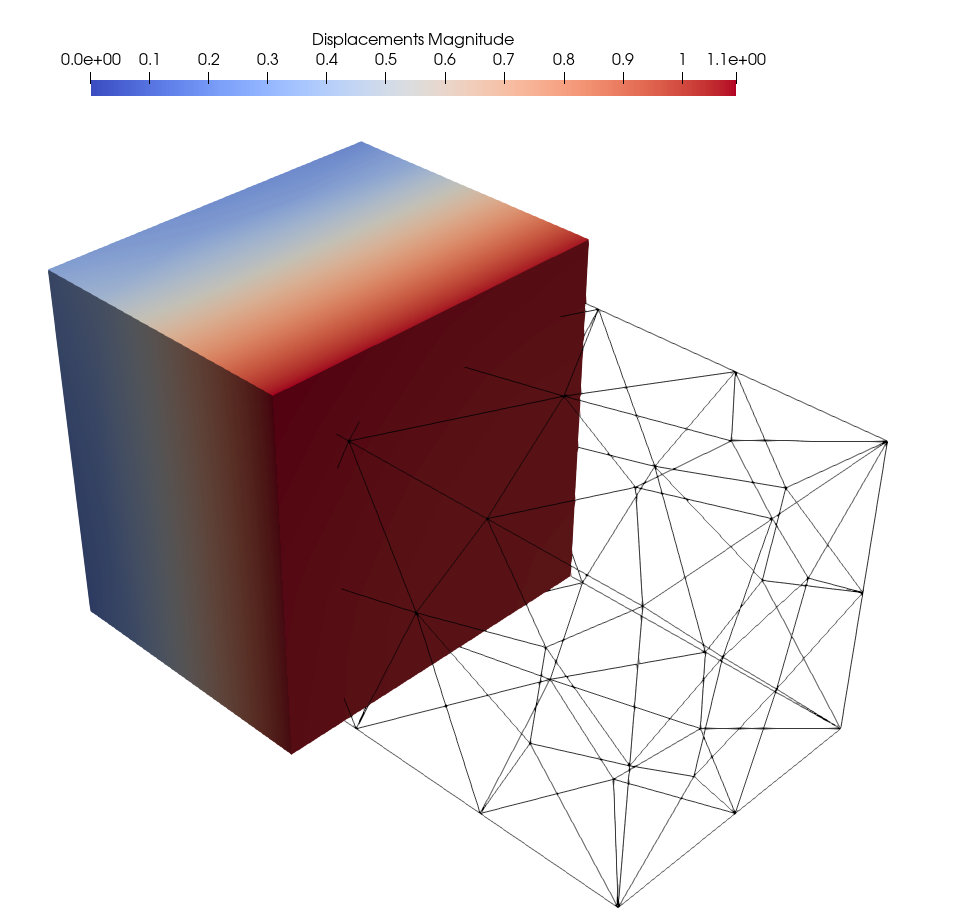
\includegraphics[width=\textwidth]{Figures/Example1.png}
	\caption{System with an applied load.}
	%\label{fig:image2}
	\end{subfigure}
	\caption{Uniaxial problem simulated and solved in \texttt{ONSAS.m}.}
	\label{fig:uniaxial_model}
\end{figure}


\subsection{Composed Cantilever Model}
Our composed cantilever model consists of two prisms made of different materials, denoted as $1$ and $2$, for which the elastic moduli and Poisson ratios are $E_1, \nu_1$ and $E_2, \nu_2$, respectively. Prism $1$ is fixed by its face at the $x=0$ plane. We applied a load of $(-p_x, t_y, t_z)$ at the plane located at $x=Lx$ along the $x, y$, and $z$ axes, respectively as shown in Figure \ref{fig:composed_cantilever_model}.

\begin{figure}[ht]
	\centering
	\begin{subfigure}[b]{0.48\textwidth}
	\def\svgwidth{\textwidth}
	\input{Figures/Example2.pdf_tex}
	\caption{Reference configuration sketch.}
	\label{fig:ex1_ilus}
	\end{subfigure}
	\hfill
	\begin{subfigure}[b]{0.48\textwidth}
	\centering
	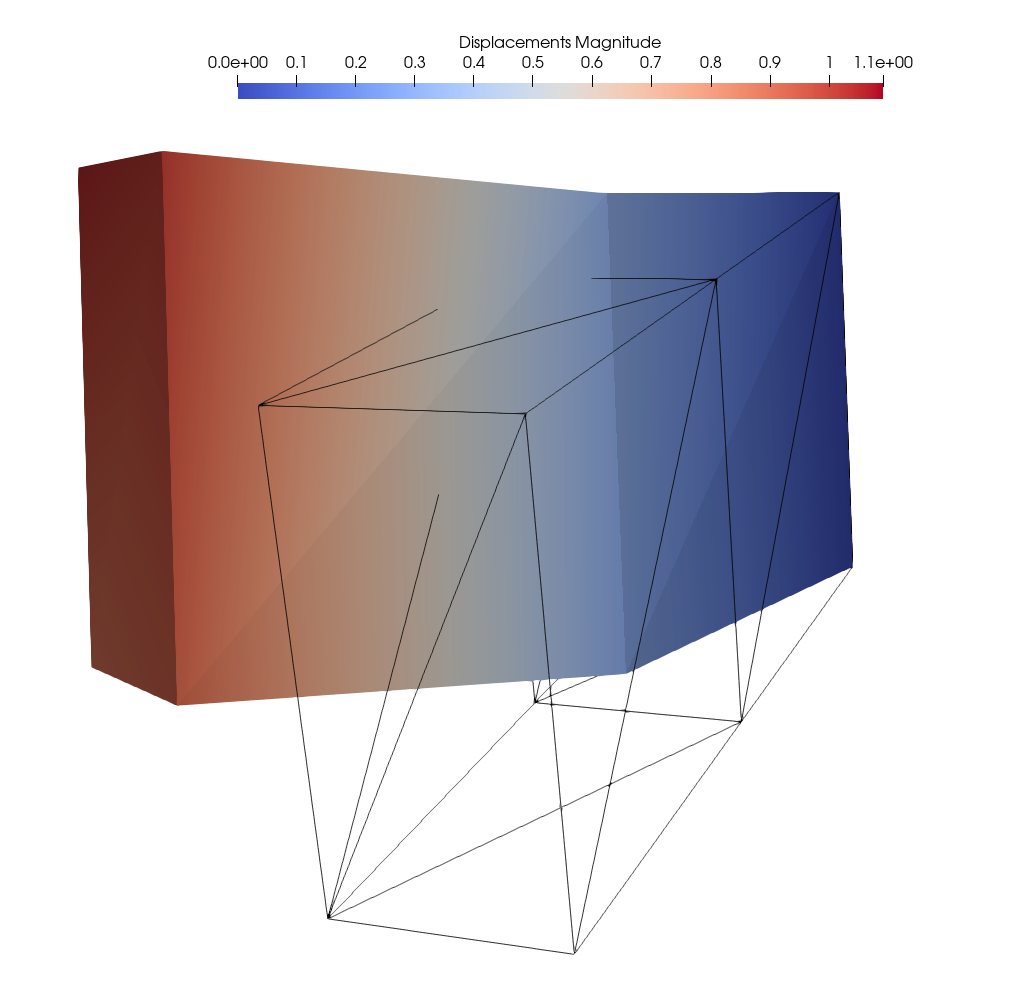
\includegraphics[width=\textwidth]{Figures/Ejemplo2.png}
	\caption{System with an applied load.}
	%\label{fig:image2}
	\end{subfigure}
	\caption{Composed cantilever problem simulated and solved in \texttt{ONSAS.m}.}
	\label{fig:composed_cantilever_model}
\end{figure}


\subsection{Bash Script}
To automate the FEM solver, we developed a bash script that generated the input files for the \texttt{ONSAS.m} \citep{ONSAS} solver and executed it repeatedly to generate a large dataset of solutions. The script also handled the output files, extracting the relevant data and formatting into a \texttt{.csv} it for further processing.

The variables swept by the script were the length of the prism $Lx$ (ranging from 1 to 3), the applied load $p$ (ranging from 0.1 to 3), and the elastic modulus of the material $E$ (ranging from 1 to 4). $Ly$ and $Lz$, were fixed at 1, and the Poisson ratio, $\nu$, was fixed at 0.3. The output of the solver was processed to obtain the displacement of the center point of the prism's face in the three dimensions.  The script generated a total of 18900 data points, which were used to train the NN.

For the composed cantilever model, we swept the variables including the length of the prism ($Lx$, ranging from 1 to 2), the applied load ($p$, ranging from 0.05 to 0.14), and the elastic moduli of each material ($E_1$ and $E_2$, ranging from 1.4 to 2.4). Fixed values were $Ly=1$,$Lz=0.5$ and  $\nu_1=\nu_2=0.3$. The output of the solver was processed to obtain the displacement of the center point of the prism's face in the three dimensions. The script generated a total of 13310 data points, which were used to train the NN.

\subsection{Neural Network}
We implemented an MLP in PyTorch to learn from the FEM solutions and solve similar mechanical problems more quickly. The MLP had two hidden layers with 20 and 10 neurons, respectively, and used the ReLU activation function. The output layer had three neurons, corresponding to the three dimensions of the displacement of the center point of the prism's face. The optimizer was Adam with a learning rate of 0.001 and 100 epochs were used. 

In the uniaxial case we used a 50/50 split for the training and validation sets, and 200 test samples using the analytic solution. For the composed cantilever case we used 1000 samples for both the training and validation sets.

We report two different loss functions: the mean squared error (MSE) and the relative MSE. The MSE is the most common loss function for regression problems, and is defined as:
\begin{equation}
\label{eq:MSE}
MSE = \frac{1}{n} \sum_{i=1}^{n} (y_i - \hat{y}_i)^2
\end{equation}
where $y_i$ is the true value and $\hat{y}_i$ is the predicted value. The relative MSE is defined as:
\begin{equation}
\label{eq:RMSE}
RMSE = \frac{1}{n} \sum_{i=1}^{n} \frac{||y_i - \hat{y}_i||_2^2}{||y_i||_2^2}
\end{equation}
The relative MSE is more useful for comparing the performance of different models, since it is normalized by the true value.

\subsection{Analytic Solution}
To compare the performance of our NN to the FEM, we computed the analytic solution to the uniaxial problem. The analytic solution is given by:

\begin{equation}
\label{eq:analytic_solution}
\boldsymbol{u} = 
(\alpha - 1)L_x \boldsymbol{e}_1 
+   
(\beta - 1) \frac{L_y}{2}  \boldsymbol{e}_2 
+   
(\beta - 1)\frac{L_z}{2} \boldsymbol{e}_3 
\end{equation}

where $\boldsymbol{u}$ is the displacement of the center point of the prism's face, $L_x$, $L_y$ and $L_z$ are the dimensions of the solid as it is shown in Figure \ref{fig:ex1_ilus}. The values of $\alpha$ and $\beta$ are obtained solving the following pair of non-linear equations:
%
\begin{eqnarray}
\alpha \left( 
\mu -  \frac{\mu}{\alpha^2} + \frac{K\beta^2}{\alpha} (\beta^2 \alpha -1)  
\right) &=& - p \\
 %
\beta \left( 
	\mu -  \frac{\mu}{\beta^2} + K (\alpha^2\beta^2 - \alpha) 
 \right) &=& 0
\end{eqnarray}
%
where  $p$ is the applied load, $K = \frac{E}{3(1 - 2\nu)}$ is the Bulk modulus and $\mu = \frac{E}{2(1 + \nu)}$ is the second Lamé parameter, $E$ is the elastic modulus and $\nu$ is the Poission's ratio. 



This allows us to generate a dataset of analytic solutions, which we can use to compare the performance of the neural network to the FEM. For doing so we used lhs to generate a Latin Hypercube Sampling of the input variables, and then computed the analytic solution for each of the 200 points in the sample.


\section{Results}
In this section, we present the results of our experiments. We compare the performance of our neural network to the FEM, and evaluate its effectiveness on a uniaxial problem and a composed cantilever problem. All the scripts used to generate the results are publicly available in the corresponding \href{https://github.com/leopoldoagorio/solid-mechanics-ML}{ GitHub repository} \footnote{\href{https://github.com/leopoldoagorio/solid-mechanics-ML}{ https://github.com/leopoldoagorio/solid-mechanics-ML} }.

\subsection{Evaluation for Uniaxial Compression}

\begin{figure}[htpb!]
	\centering
	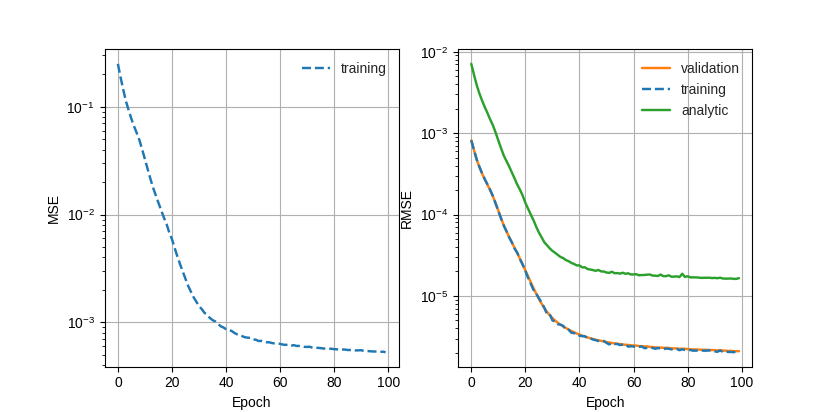
\includegraphics[width=1\textwidth]{Figures/Example1_losses.png}
	\caption{Training, validation and test loss of the neural network on the uniaxial compression/extension dataset.}
	\label{fig:train_loss}
	\end{figure}
 
Figure \ref{fig:train_loss} shows the training, validation, and test losses of our neural network on the uniaxial compression/extension dataset. The final training loss for MSE is $5.29\times10^{-4}$ and the RMSE is $2\times10^{-6}$. The final validation loss RMSE is $2\times10^{-6}$, and the final analytic loss RMSE is $1.7\times10^{-5}$.
%\begin{itemize} \item Final training loss MSE 0.000529
%	\item Final training loss RMSE 0.000002
%	\item Final validation loss RMSE 0.000002
%	\item Final analytic loss RMSE 0.000017
%	\item RMSE extrapolation error for (Lx, E, p) = (4.00, 0.50, 3.50): is 0.067281 \item MSE extrapolation error for (Lx, E, p) = (4.00, 0.50, 3.50): is 0.946485 m$^2$ 
%\end{itemize}
We also evaluated the ability of our model to extrapolate beyond the parameters in the training set. When we measured the RMSE extrapolation error for $(Lx, E, p) = (4.00, 0.50, 3.50)$, we found it to be $6.7\times10^{-2}$, while the MSE extrapolation error was $9.5\times10^{-1}$ $m^2$. Since the variation range for the training parameters was $(Lx, E, p) = (1 \hdots 3, 1 \hdots 4, .1 \hdots 3)$, these results show that our neural network was able to extrapolate to a point that was not in the training set, with an error of 6.7 of the true value.

\subsection{Evaluation on Cantilever Model}
For the case of the composed cantilever model, the training, validation and test loss is shown in Figure \ref{fig:composed_cantilever_loss}. As we can see, the training loss decreases rapidly during the first few epochs and then levels off. 

\begin{figure}[ht]
\centering
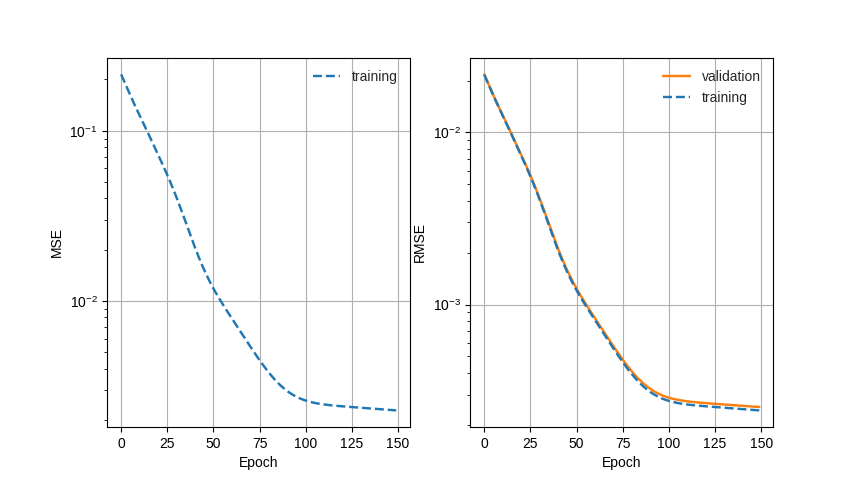
\includegraphics[width=1\textwidth]{Figures/Example2_losses.png}
\caption{Training, validation and test loss of the neural network on the composed cantilever dataset.}
\label{fig:composed_cantilever_loss}
\end{figure}


Figure \ref{fig:composed_cantilever_loss} shows the training, validation, and test losses of our neural network on the cantilever model. The final training loss for MSE is $2.3\times10^{-3}$ and the RMSE is $2.4\times10^{-4}$. The final validation loss RMSE is $2.5\times10^{-4}$, and the final analytic loss RMSE is $2.9\times10^{-4}$.

We also evaluated the ability of our model to extrapolate beyond the parameters in the training set. When we measured the RMSE extrapolation error for $(Lx, E1, E2, p) = (1.50, 1.3, 1.3, 0.10)$, we found it to be $0.21$. Since the variation range for the training parameters was $(Lx, E1, E2, p) = (1 \hdots 2, 1.4 \hdots 2.4, 1.4 \hdots 2.4, 0.05 \hdots 0.14)$, these results show that our neural network was able to extrapolate to a point that was not in the training set, with an error of $21 \%$ of the true value. 
%$6.7\times10^{-2}$, while the MSE extrapolation error was $9.5\times10^{-1}$ $m^2$. Since the variation range for the training parameters was $(Lx, E, p) = (1 \hdots 3, 1 \hdots 4, .1 \hdots 3)$, these results show that our neural network was able to extrapolate to a point that was not in the training set, with an error of 6.7 of the true value.

%\begin{itemize}
%\item Final training loss MSE 0.002276  
%\item Final training loss RMSE 0.000243  
%\item Final validation loss RMSE 0.000254  
%\item Final test loss RMSE 0.000287  
%\item RMSE extrapolation error for (Lx, E1, E2, p) = (1.50, 1.20, 1.20, 0.16): is 0.672594
%\end{itemize}

\section{Conclusion}
In this project, we developed a pipeline for generating a dataset of FEM solutions to simple solid mechanical problems, and used this dataset to train a neural network to predict the same displacement field at control nodes more quickly.
%
Our experiments showed that our approach was effective, with the neural network achieving low losses on both the training and test datasets, and closely matching the theoretical curve for uniaxial compression. We also demonstrated that our approach has the potential to be extended to more complex mechanical problems, as shown by our evaluation on a cantilever model. 

One advantage of our implementation is its simplicity and scalability. By using a relatively simple mechanical problem, we were able to develop a pipeline that can be easily scaled to more complex problems. Additionally, the use of a neural network allows for faster computation times than the traditional FEM method. This has the potential to significantly reduce computational costs on any numerical processes that rely on FEM simulations, such as material identification algorithms for tissue disease diagnostics problems and stress CAD for manufacturing. However, as it is shown in the results, predictions for material properties outside the train space, may lead to higher error rates. 


In conclusion, this project demonstrates the effectiveness of using a neural network to solve simple mechanical problems. By developing a faster surrogate model, we have shown the potential to significantly improve the efficiency of solving such problems, with broader implications for the engineering design process. Future work includes scaling our approach to more complex mechanical problems and evaluating its effectiveness on a larger dataset.

\bibliography{amcapaper}
\end{document}
